\chapter{REFERENCIAL TEÓRICO}

\section{Desenvolvimento Rural Sustentável}

Definir o desenvolvimento do meio rural sustentável requer um considerável esforço observacional e prático, pois, este ambiente vem sofrendo profundas transformações em suas demandas e necessidades, o desenvolvimento que antes se apresentava majoritariamente como produção de subsistência, hoje dá lugar a um complexo sistema agroindustrial \cite{bastos_determinantes_2018} e social. É importante neste sentindo compreender que definir o desenvolvimento rural com apenas um conceito seria uma proposição simplista do contexto de desenvolvimento rural. Partindo da definição de consequência de ações governamentais definidas por \citeonline{navarro_desenvolvimento_2001} como "ações práticas", este autor descreve que o:

\begin{citacao}
“[...] Desenvolvimento rural, portanto, pode ser analisado a posteriori, neste caso se referindo às análises sobre programas já realizados pelo Estado (em seus diferentes níveis) visando a alterar facetas do mundo rural a partir de objetivos previamente definidos. Mas pode se referir também à elaboração de uma "ação prática".
\end{citacao}

O desenvolvimento rural também pode ser compreendido por um conceito mais regional definido como "Desenvolvimento Local". Tal expressão é recente e deriva de iniciativas de mobilização organização social no sentido de promover uma maior representação dos diferentes atores sociais no processo de desenvolvimento. E que o Estado assume papel de agente facilitador desse processo de descentralização das políticas públicas  para ser democrático, a transparência de suas instituições, o equilíbrio das forças exercidas pelas diferentes correntes de interesse e o compromisso com a qualidade de vida na população afetada \cite{campanhola_diretrizes_2000}. Tal conceito demonstra o espaço rural como um local ideal para a promoção de políticas de inovação e a construção de padrões inovadores na relação entre populações e instâncias públicas, numa tentativa de rompimento com a dominação, que parte de baixo para cima. Neste contexto, surge as Organizações Não Governamentais (ONGs) que buscam garantir a participação da população local, e fazer valer tais mudanças atuando normalmente em ambientes geograficamente mais restritos (região rural, povoados ou municípios), \cite{assis_agricultura_2005, campanhola_diretrizes_2000}.

E por fim, este trabalho está direcionado em estudos relacionados ao Desenvolvimento Rural Sustentável. Anteriormente, o conceito de Desenvolvimento Rural Sustentável era denominado por "Progresso Rural", pois, havia um entendido genérico como sentido parcial e prático de “melhoramento do ambiente” \cite{almeida_da_1995}. Entretanto, torna-se imprescindível destacar que, o desenvolvimento sustentável no meio rural não pode ter suas bases de compreensão apenas no progresso econômico, local ou regional. Se mostra de suma importância entender que para compreender a sustentabilidade é necessário ter um olhar sistêmico que permeie todo o processo, envolvendo diversas dimensões, dentre as quais se destacam a econômica, a sociocultural, a político-institucional e a ambiental \cite{vieira_politica_2015}, a ação de desenvolvimento sustentável é por um lado fruto do desenvolvimento social, por outro lado, esta ação contribui com o desenvolvimento da sociedade de forma autossustentável, ao introduzir inovações anti-predatórias, ao satisfazer demandas específicas tendo como base a economia circular e ao tornar mais densas as redes de cooperação buscando a autossuficiência consciente, satisfazendo as necessidades no presente, sem comprometer a capacidade das gerações futuras de suprir suas próprias necessidades \cite{onu_sustainable_2016}.

No Brasil, o desenvolvimento rural propriamente dito teve início com a política de “Intensificação verde” por meio da revolução verde, plano político que teve força de ação iniciando nos anos 60. Tal política era baseada em subsídios de créditos que buscava o estímulo à produção agrícola em larga escala principalmente de \textit{commodities}, do mesmo modo impulsionava o crescimento do setor de transporte com expansão da malha rodoviária, as políticas de crédito rural, os preços mínimos, as pesquisas e extensão rural \cite{kageyama_o_1990}. Os incentivos e créditos que de fato chegaram ao campo foram em sua maioria, utilizados por empresas de maquinários e de insumos industriais para uso agrícola \cite{strassburg_producao_2015}, impulsionando apenas o aumento da produção em escala industrial, deixando de lado as preocupações com a manutenção dos recursos limitados no campo e a capacidade de escalabilidade dos pequenos produtores.

Tal desenvolvimento teve como ponto positivo o estreitamento das fronteiras entre o meio rural e o meio urbano, tornando-as cada vez mais tênues e difusas \cite{freitas_mudancas_2012}, já que a sociedade civil emerge como protagonista desse processo de construção dos pilares para um desenvolvimento mais responsável e abrangente \cite{de_souza_empreendedorismo_2016}. 

Desta forma, os produtores agrícolas atuais além de suprir as necessidades alimentares da população, se desenvolve ainda mais para produzir particularidades para população urbana, como produtos com maior qualidade, rapidez e efetividade na entrega, volume cada vez maior, entre outras. Atualmente ao pensar em tecnologias inovadoras para o campo, é necessário compreender as necessidades do meio urbano e as possíveis capacidades do meio rural, de maneira que este se mantenha autossustentável em todas as características ambientais, sociais e culturais, sendo de suma importância a compreensão do que de fato venha a ser rural e como construir sua sustentabilidade. As soluções propostas para superar esses desafios devem não apenas considerar a maneira como os alimentos são produzidos, mas também ponderar sobre preocupações sociais, ambientais e econômicas \cite{kamble_achieving_2020}. 

O rural deve ser visto segundo \cite{kageyama_desenvolvimento_2008} como, uma amálgama de práticas heterogêneas, estilos mutuamente contrastantes, tendências de desenvolvimento divergentes, posições hegemônicas e mudanças quase subterrâneas que, a princípio, são praticamente imperceptíveis, mas que, por fim, podem mudar todo o sistema de produção. Compreender a complexidade do rural se faz necessário uma vez que a simples padronização do ambiente é um conceito reducionista do campo, uma maneira concisa do que ocorre no rural \cite{van_der_ploeg_trajetorias_2011}. 

O empreendedorismo é uma das ferramentas possíveis para promoção de desenvolvimento do campo e que considera suas complexidades,  \citeonline{autio_retaining_2016} afirmam que um euro de financiamento público para as iniciativas em empreendedorismo gerou 1,11 euro de crescimento das vendas excedentes. Para que seja aplicado corretamente, se faz necessário compreender melhor o empreendedorismo sustentável como também a aplicação prática no meio rural. 

Segundo \citeonline{dornelas_como_2003}, o empreendedorismo significa fazer algo novo, diferente, mudar a situação atual e buscar, de forma incessante, novas possibilidades de negociações, tendo como foco a inovação e a criação de valor, outrossim, \citeonline{leite_aprendizagem_2015} trata o empreendedorismo como  um  processo,  que se concentra em iniciar  e  gerir  empreendimentos,  isto  é,  o conjunto  de  conceitos,  métodos,  instrumentos  e  práticas  relacionadas  com  a criação, implantação  e  gerenciamento de novas  empresas  ou organizações.

Existem diversas definições de empreendedorismo, mas a essência resume-se na inovação, ou seja, criação de algo novo ou modificação de algo buscando uma nova aplicação, empregando os recursos disponíveis de forma criativa, assumindo riscos calculados e buscando oportunidades, é um processo de criação de um negócio de valor com recursos limitados tornando-o capitalizável e economicamente viável \cite{costa_empreendedorismo_2006, stevenson_new_1989, lopes_educacao_2010}. Apesar dessa diversidade conceitual, a ideia de empreendedorismo tem sido predominantemente associada às concepções de progresso e tecnologia usual deixando de lado o campo e nele suas aplicações práticas.  

O intenso debate sobre desenvolvimento da agricultura brasileira de forma sustentável em consonância com assuntos econômicos de interesse nacional torna o tema desta pesquisa oportuno e atual, haja vista que a agricultura no Brasil corresponde a 19\% do total das exportações no ano de 2018 \cite{mdic_comex_2019}. Entretanto, este meio de produção convive com a limitação dos recursos naturais \cite{jacobi_meio_1999}, levando ao Estado pensar em políticas públicas que busquem soluções para as demandas tecnológicas surgidas no meio rural, e gerar profissionais capazes de compreender a complexidade da intensa produção no campo mantendo o ritmo constante das mudanças tecnológicas ao mesmo tempo, do uso de limitados recursos naturais \cite{costa_dinamica_2016}.
No alcance desse modelo sustentável, um profissional empreendedor deve ser preparado desde a academia por meio da educação empreendedora de modo que seja capaz de melhorar o desempenho produtivo \cite{da_silva_qualidade_2017}, a capacidade competitiva, a melhoria da segurança alimentar do país \cite{hoffmann_brasil_2014} e, ao mesmo tempo garantir a perpetuação da manutenção do meio ambiente, e não apenas replicar novos padrões de produção e distribuição de bens e serviços e do uso dos recursos naturais, além disso, este profissional deve ser capaz de inovar \cite{morais_empreendedorismo_2018}.

Sobre tais bases, conclui-se que o desenvolvimento do campo de forma tradicional dispõe de poucas hipóteses, além da alternativa de uma prática intensiva em capital e exploração dos recursos naturais, cuja intensificação e amplitude pode levar a escassez dos meios \cite{costa_agrarian_2016}. 


\section{Agritechs}

Atualmente passamos por uma fase muito expressiva da disseminação do empreendedorismo no Brasil e no mundo, tendo como exemplo o crescimento das "Startups" saindo de 2519 em 2012, para 12.815 na presente data, \cite{abstartups_startupbase_2019}. A velocidade do desenvolvimento e conexões das negociações antes realizadas de pessoa a pessoa, atualmente passa pelo campo da automação e digitalização aumentando a velocidade da inovação interferindo na relação entre pessoas e produtividade \cite{campos_o_2016}. 

Independentemente do tamanho e demanda que venha a ter o proprietário do comércio, o desempenho negocial do empreendimento depende da capacidade de adaptação e resiliência  do administrador, assim também são os negócios no meio rural. O grande produtor objetivando o desenvolvimento de capital utiliza-se de um vasto corpo de recursos humanos e tecnológico, já os pequenos produtores muitas vezes dependem apenas deles mesmos, sendo proprietário e administrador, ou quando exige a possibilidade de contratação passa a depender de apenas um profissional responsável por lidar com todos os entraves da produção agrícola e as mudanças constantes do meio rural \cite{soares_relacao_2017}. Uma das alternativas possíveis para reduzir os riscos de se manter em todas as funções citadas em apenas um profissional, é o investimento em tecnologia e inovação tais como: sementes melhoradas, adubação agrícola mais eficiente, centros coletivos de pesquisa direcionadas ao campo (Universidades e empresas) \cite{bochi_dorneles_coletivos_2014, gomes_inovacao_2014} e pequenas empresas prestadoras (startups) de serviços ou nichos do mercado rural. Estes negócios objetivam a melhoria de determinada área agropecuária \cite{junior_agtechs:_2019} ou necessidade do negócio, de forma efetiva e economicamente viável. Elas surgiram por meio das oportunidades que os negócios e as necessidades lhes apresentaram. As Startups transformam as necessidades e ideias em negócio viável e sustentável, ligam-se muito ao meio rural já que para obter sucesso e alcançar o crescimento rápido na produtividade agrícola é necessária uma capacidade de gerar tecnologias adaptativas e ecológicas \cite{contini_hayami_2019}.

O modo como se processa a diversificação tecnológica no campo relaciona-se diretamente com o desenvolvimento e a adaptação de novas tecnologias agrícolas e a diversidade das condições socioeconômicas e ambientais \cite{fen-azmeyer_o_2019}. Neste ambiente de cocriação surge as Startups direcionadas à agricultura, tais empresas de base tecnológica são focadas em soluções para o agronegócio, muitas vezes são referenciadas como um setor \textit{Agtech} \cite{blanco_agtechs:_2019}.

Dentre o espectro de novos empreendimentos, os mais comuns para o agronegócio no Brasil são: \textit{Business to Business} (B2B), \textit{Business to Consumer} (B2C), \textit{Business to Business to Consumer} (B2B2) e o \textit{Direct to Consumer} (D2C). Segundo \citeonline{junior_agtechs:_2019} e \cite{abstartups_startupbase_2019}, as principais  áreas de atuação destas Startups são as áreas de: Biotecnologia de Alimentos inovadores atendendo tanto B2B quanto B2B2C, Marketplace do agronegócio (B2B2C), Bioenergia e Biomateriais (B2B), indústria de Software como Serviço SaaS (B2B).


\section{Comportamento Empreendedor e Educação empreendedora}


A Intenção empreendedora (IE) é a matriz de toda atividade e desenvolvimento ao empreendedorismo e surgimento de novos negócios, esta intenção pode ser vista como o primeiro passo no processo empreendedor \cite{zhao_relationship_2010, shirokova_exploring_2016}. Estudos recentes demonstram que a IE para abertura de negócios vai muito além do dualismo oportunidade-necessidade, ou seja, a criação e/ou descoberta de oportunidades, faz parte também o medo do desemprego, e a  incapacidade de adaptação as mudanças técnicas e tecnológicas especialmente em países em desenvolvimento \cite{vale_motivacoes_2014}. As motivações extrapolam a lógica binária oportunidade/necessidade, e agrupam-se em seis componentes: identificação  de  oportunidade;  atributos/expectativas pessoais; ambiente  externo em particular associado ao mercado de trabalho; influência  de  terceiros, insatisfação com emprego; influência familiar, \cite{vale_motivacoes_2014, rodrigues_intencao_2019,ferreira_intencao_2017}.

Buscando lidar com tais variáveis, conceitos e ferramentas psicológicas devem ser aplicados não apenas a ambientes empresariais, mas durante toda a formação acadêmica, em combinação com um profundo conhecimento de pesquisa e negócios \cite{zhao_relationship_2010} já que, a existência do empreendedorismo reside em tomadas de decisões inovadoras, das quais não se separam das características intrínsecas do individuo e suas experiências durante sua construção pessoal, por meio de trocas sociais \textit{networking} \cite{de_souza_alencar_intencao_2019}.

A inovação, a propagação da inovação e o surgimento de novos empreendimentos, em muitos países, são tidos como importantes sinais para o crescimento e recuperação de crises econômicas \cite{silva_mudancestrutural_2017}, tais sinais de desenvolvimento estão ligados diretamente ao desenvolvimento intelectual do capital humano. Segundo o \cite{reis_capital_2017} o capital humano é o insumo fundamental da Pesquisa e Desenvolvimento (P\&D), e a P\&D é a condição \textit{sine qua non} para a geração e a intensidade de novidades, e as inovações catalisam e dinamizam o processo de crescimento econômico.

O Investimento no  capital  humano desde a formação acadêmica permite também o surgimento de melhorias no ambiente laboral e aumenta os níveis de produtividade e renda dos futuros profissionais \cite{macedo_capital_2019}. Até pouco tempo, os currículos educacionais nas escolas e cursos relacionados a administração no Brasil focavam quase que totalmente ao atendimento às necessidades do mundo corporativo, deixando de lado o fator (criatividade e inovação), buscavam profissionais técnicos na prevenção de riscos ao invés de formar líderes criativos que criem estratégias de prevenção, assumam riscos \cite{sanna_evolution_1999} e os solucione, além da manipulação do ambiente externo, gerenciar o crescimento e a inovação em pequenas e médias empresas exige que os novos empreendedores possuam uma capacidade distinta de tomar e implementar decisões e fortes habilidades de liderança \cite{palmer_chip_2019}. Parece, deste modo, interessante investigar a figura do aluno como sujeito potencialmente empreendedor, como uma pessoa capaz de identificar oportunidades, criar negócios, e pode reunir os recursos necessários face ao risco e incerteza, \cite{pietrovski_alise_2019}.


O mercado econômico emergente, as necessidades de entregas urgentes e a redução cada vez maior das ofertas de emprego levou os centros de ensino a iniciarem o desenvolvimento deste conteúdo disciplinar e os demais conteúdos relacionados. No início dos anos 80 o empreendedorismo estava diretamente ligado ao desenvolvimento econômico e à criação de postos de trabalho em um país \cite{rodrigues_intencao_2019}, passando a ser visto como importante fator a ser explorado nas comunidades acadêmicas. É nesse contexto que surge o ensino do empreendedorismo no Brasil tendo como precursor o Professor Ronald Degen \cite{degen_o_1989} na Escola de Administração de Empresas de São Paulo (EAESP) pertencente a Fundação Getúlio Vargas (FGV), em 1981. É vasta a literatura voltada para o tema, podemos destacar as pesquisas de: \citeonline{dolabela_oficina_1999}; \citeonline{duarte_sesi_2004}; \citeonline{pires_empreendedorismo_2006}; \citeonline{ramos_o_2005}, \citeonline{branca_terra_o_2006}, entre outros. A Tabela \ref{tabela_1} desenvolve um recorte histórico do ensino da área no Brasil, tendo como corte temporal 1980 a 2007, segundo \cite{fernandes_breve_2013}. 



\begin{longtable}{lp{11cm}}

\caption{\textbf{Histórico do Ensino de Empreendedorismo no Brasil}}\label{tabela_1} \\ \hline \hline


\hline \multicolumn{1}{p{2cm}}{\textbf{Ano}} & \multicolumn{1}{p{11cm}}{\textbf{Ocorrência}}\\ \hline 

\endfirsthead


\multicolumn{2}{c}%

{{\bfseries \tabname \ \thetable{} -\ \textbf{Continuação}}}\\

\hline \multicolumn{1}{p{2cm}}{\textbf{Ano}} & \multicolumn{1}{c}{\textbf{Ocorrência}}  \\ \hline 

\endhead

\hline \multicolumn{2}{r}{{\textbf{Continua}}} \\ \hline

\endfoot
\hline \multicolumn{2}{r}{{\textbf{Continua}}} \\ \hline

\endfoot
\hline \multicolumn{2}{r}{{\textbf{Conclusão}}} \\ \hline
\hline \hline

\endlastfoot


1980 & Fundação Getúlio Vargas - FGV implanta o ensino formal de empreendedorismo no Brasil;  \\\\\hline
1980 & A Universidade de São Paulo - USP institui polo de ensino de empreendedorismo;  \\\\\hline
1981 & O Professor Ronald Degen leciona a disciplina “Criação de Negócios”  \\\\ \hline
1984 & O Professor Sílvio dos Santos, da USP leciona disciplina referente à criação de novas \\\\ \hline
1991 & A Professora Ofélia Sette Torres funda o Centro de Empreendedorismo;  \\\\\hline
1991 & É introduzido no Brasil o Programa Empretec, da Organização das Nações Unidas - ONU, para
capacitar empreendedores;  \\\\\hline
1993 & O Empretec passa a ser coordenado pelo Sebrae no Brasil;  \\\\ \hline
1996 & O Professor Paulo Goldsmith, coordena a versão brasileira da competição internacional Global Moot Corp, realizada pela Universidade do Texas desde 1984. Em 2001 essa competição foi aberta a todas as escolas da América Latina, passando a se chamar Latin America Moot Corp;\\\\ \hline
1999 & Lançamento do livro “O Segredo de Luísa”, do Professor Fernando Dolabela, renomado
especialista em educação empreendedora no Brasil e criador da Pedagogia Empreendedora;  \\\\ \hline
2000 & Os professores Tales Andreassi e Marcelo Aidar passam a ministrar curso de empreendedorismo
na EAESP;  \\\\ \hline
2002 & O Professor José Antônio Lerosa de Siqueira funda na USP o Centro Minerva de Empreendedorismo;  \\\\\hline 
 2005 & É realizada a primeira Semana do Empreendedorismo pelo Centro de Empreendedorismo e Novos Negócios da FGV. Atualmente o centro é o responsável pela Latin America Moot Corp e pela competição Sumaq16 de empreendedorismo social;  \\\\ \hline 
 2007 & A FGV é pioneira ao estabelecer como obrigatórias disciplinas que tratem do tema empreendedorismo nas grades curriculares dos cursos de graduação em administração pública e de empresas da EAESP; \\\\ \hline

\end{longtable}
 \fonte{\cite{almeida_aprendizagem_2019}}


Fica nítido que a preocupação com o ensino de empreendedorismo está saindo de sua fase embrionária e se consolidando nos principais  centros de graduação e pós-graduação, nos mais diversos segmentos de formação desde cursos de engenharia, passando por desenho industrial, até o turismo \cite{henrique_praticas_2008}. A educação empreendedora como investimento ao capital humano, a além de fortalecer a criação de produtos e a dinamização de atividades econômicas, torna-se uma possibilidade de combater o desemprego \cite{morais_empreendedorismo_2018} e a redução das jornadas de trabalho e custos com materiais. Para \citeonline{schaefer_formacao_2017}, o indivíduo empreendedor é o ator capaz de inovar no processo evolutivo do mundo contemporâneo, capaz de resolver problemas e absorver oportunidades, atribuindo-se este sujeito como causa da mudança, e capaz de lidar com as constantes inversões do mercado econômico. Desta forma se faz necessário um robusto incentivo ao empreendedorismo e a promoção de sua cultura visto que, a criação de negócios está diretamente ligada à ação empreendedora, processo dinâmico que possibilita a desenvolvimento de empregos e riquezas, impactando na prosperidade de diversas regiões do Brasil \cite{leite_aprendizagem_2015}, assim como no Brasil existe uma progressiva necessidade do ensino ao empreendedorismo correto e escalável, um país que segue um constante crescimento de empregos informais, país que apresentou no ano de 2019 um contingente de pessoas que conseguiram trabalho no período está em condição de informalidade, que atingiu um recorde da série histórica, iniciada em 2012, chegando a 41,4\% de recursos humanos ocupados ocupados no Brasil \cite{ibge_informalidade_2019}, como também uma taxa crescente de desocupação nas idades iniciais de empregabilidade (14 aos 24 anos) desde 2012, dados obtidos na Pesquisa Nacional por Amostra de Domicílios Contínua - PNAD Contínua \cite{ibge_instituto_brasileiro_de_geografia_e_estatistica_pesquisa_2019}, dados podem ser vistos na figura \ref{figura_2}, mesmo os alunos graduados ainda apresentam lacunas de formação em seu potencial empreendedor e que cabe às universidades criar processos de ensino e aprendizagem que preencham esses espaços \cite{pietrovski_alise_2019}.


\begin{figure}[!htb]
\centering
\caption{\textbf{Taxa de desocupação por idade, 1º trimestre 2012 - 3º trimestre 2019}}
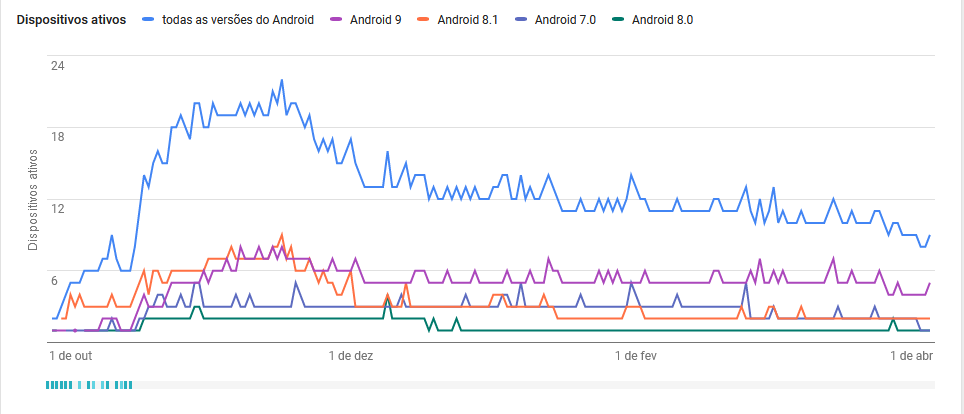
\includegraphics[scale=0.25]{Imagens/taxa_desocupacao.png}
\fonte{\citeonline{ibge_instituto_brasileiro_de_geografia_e_estatistica_pesquisa_2019}}
\label{figura_2}
\end{figure}
\newpage

Com as universidades e institutos de ensino superior sendo reconhecidamente contextualizados como promotores da inovação no Brasil, país que configura o 13.º lugar entre os maiores produtores de publicações de pesquisa (\textit{papers}) e inovação a nível mundial, \citeonline{clarivate_analytics_web_of_research_2017}. 
O novo paradigma educacional, portanto, situa as instituições de ensino superior no campo da promoção do empreendedorismo direcional e sistemático, assim como o comportamento empreendedor, educação empreendedora disciplinada mostra-se eficaz no tocante ao surgimento das inovações, direcionadas e a promoção da identidade empreendedora para novos negócios, \cite{jain_academics_2009} já que a universidade vem a ser um local privilegiado do saber, da liberdade acadêmica e da experimentação científica tem o poder de ‘oficializar’ o empreendedorismo como um conteúdo de conhecimento é uma ferramenta capaz de gerar inovações \cite{dolabela_oficina_2008}. 


Atualmente, diversos tipos de métodos e ferramentas de ensino podem ser utilizados para auxiliar o docente e, consequentemente, motivar os estudantes em sua experiência na aprendizagem. Para atingir os objetivos da educação empreendedora, é preciso promover reflexões nos campos do ensino, formação de professores, uso dos recursos e infraestrutura \cite{marques_experiencia_2019}, já que o desenvolvimento do interesse ao empreendedorismo envolve diversos conteúdos de aprendizado, é necessário organizar as metodologias e suas aplicações pedagógicas \cite{rocha_avaliacao_2014}. O mesmo autor elencou os Principais Métodos, Técnicas e Recursos Pedagógicos no Ensino do Empreendedorismo. 



\begin{longtable}{p{3.5cm}p{11.0cm}}

\caption[\textbf{Principais  Métodos, Técnicas e Recursos Pedagógicos no Ensino de Empreendedorismo}]{\textbf{Principais  Métodos e Recursos Pedagógicos no Ensino de Empreendedorismo}} 
\label{tabela_2} \\


\hline \hline \multicolumn{1}{p{3.5cm}}{\textbf{Métodos, Técnicas e Recursos}} & \multicolumn{1}{c}{\textbf{Aplicações}}\\ \hline 

\endfirsthead


\multicolumn{2}{c}%

{{ \bfseries \tablename \ \thetable{} - \ \textbf{Continuação}}}\\

\hline \multicolumn{1}{p{3.5cm}}{\textbf{Métodos, Técnicas e Recursos}} & \multicolumn{1}{c}{\textbf{Aplicações}}  \\ \hline 

\endhead

\hline \multicolumn{2}{r}{{\textbf{Continua}}} \\ \hline

\endfoot
\hline \multicolumn{2}{r}{{\textbf{Continua}}} \\ \hline

\endfoot
\hline \multicolumn{2}{r}{{\textbf{Conclusão}}} \\ \hline
\hline \hline

\endlastfoot

Aulas expositivas & Transferir conhecimentos sobre o Empreendedorismo, as características pessoais do empreendedor, os processos de inovação, fontes de recursos, financiamentos e aspectos legais de pequenas empresas.  \\

Visitas e contatos com empresas & Estimular o \textit{network} e incitar o estudante a sair dos limites da IES para entender o funcionamento de mercado na vida real. Desenvolver visão de mercado.  \\

Plano de negócios & Desenvolver as habilidades de planejamento, estratégia, marketing, contabilidade, recursos humanos, comercialização. Desenvolver a habilidade de avaliação do novo negócio, analisando o impacto da inovação
no novo produto ou serviço. Construir habilidade de avaliar e dimensionar riscos do negócio pretendido. \\ 

Estudos de situações problemas & Construção da habilidade de pensamento crítico e de avaliação de cenários e
negócios. Desenvolver a habilidade de interpretação e definição de contextos associados ao Empreendedorismo. \\ 

Trabalhos teóricos em grupo & Construção da habilidade de aprender coletivamente. Desenvolver a
habilidade de pesquisar, dialogar, integrar e construir conhecimentos,
buscar soluções e emitir juízos de valor na realização do documento escrito. \\ 

Trabalhos práticos em grupo & Construção da habilidade de atuar em equipe. Desenvolver a habilidade de planejar, dividir e executar tarefas em grupo, de passar e receber críticas construtivas. Ampliar a integração entre o saber e o fazer.  \\ 

Grupos de discussão & Desenvolver a habilidade de testar novas ideias. Desenvolver a capacidade de avaliar mudanças e prospectá-las como fonte de oportunidades. \\ 
 
\textit{Brainstorming}  & Construção da habilidade de concepção de ideias, prospecção de
oportunidades, reconhecendo-as como oportunidades empreendedoras. \\ 


Seminários e palestras com empreendedores & Transferir conhecimentos das experiências vividas por empreendedores
desde a percepção e criação do produto, abertura do negócio, sucessos e
fracassos ocorridos na trajetória empreendedora. \\ 

Criação de empresa & Transpor as informações do plano de negócios e estruturar os contextos necessários para a formalização. Compreender várias etapas da evolução da empresa. Desenvolver a habilidade de organização e planejamento operacional. \\ 

Aplicação de provas dissertativas & Testar os conhecimentos teóricos dos estudantes e sua habilidade de
comunicação escrita. \\ 

Atendimento individualizado & Desenvolver a habilidade de comunicação, interpretação, iniciativa e
resolubilidade. Aproximar o estudante do cotidiano real vivido nos pequenos negócios. \\ 

Trabalhos teóricos individuais & Construção da habilidade de concepção de conhecimento individualizado,
estimulando a autoaprendizagem. Induzir o processo de autoaprendizagem. \\ 

Trabalhos práticos individuais & Construção da habilidade da aplicação dos conhecimentos teóricos
individuais, estimulando a autoaprendizagem. Estimular a capacidade
laboral e de auto realização. \\ 

Criação de produto & Desenvolver habilidade de criatividade, persistência, inovação e senso de
avaliação. \\ 

Filmes e vídeos & Desenvolver a habilidade do pensamento crítico e analítico, associando o
contexto assistido com o conhecimento teórico. Estimular a discussão em grupo e o debate de ideias. \\ 

Jogos de empresas e simulações & Desenvolver a habilidade de criar estratégias de negócios, solucionar
problemas, trabalhar e tomar decisões sob pressão. Aprender pelos próprios erros. Desenvolver tolerância ao risco, pensamento analítico, comunicação intra e intergrupais. \\ 

Sugestão de leituras & Prover ao estudante teoria e conceitos sobre o Empreendedorismo. Aumentar a conscientização do ato empreendedor. \\ 
Incubadoras & Proporcionar ao estudante espaço de motivação e criação da nova empresa, desenvolvendo múltiplas competências, tais como habilidades de liderança, organizacionais, tomada de decisão e compreender as etapas do ciclo de vida das empresas. Estimular o fortalecimento da network com financiadores, fornecedores e clientes. \\

Competição de planos de negócios & Desenvolver habilidades de comunicação, persuasão e estratégia.
Desenvolver capacidade de observação, percepção e aplicação de melhorias no padrão de qualidade dos planos apresentados. Estimular a abertura de empresas mediante os planos vencedores. \\ 

\end{longtable}
\fonte{\cite{rocha_avaliacao_2014}}




Os centros de ensino devem contribuir para o desenvolvimento da “cultura empreendedora” por meio da “educação empreendedora ativa” \cite{tscha_empreendendo_2014}, que incentive tanto docentes quanto aos discentes, “despertarem dentro de si o espírito empreendedor e a explorar o espaço potencial para o empreendedorismo, transformando realidades por meio dos empreendimentos que podem desenvolver economicamente e socialmente um país e uma sociedade” \cite{tscha_empreendendo_2014}. Uma vez que, a cultura empreendedora depende diversos fatores influenciáveis ao longo do aprendizado e vida. \cite{dornelas_empreendedorismo:_2005} explica que  empreender segue fluxo um definido que depende de fatores determinantes durante a construção correta e satisfatória da cultura empreendedora. Alguns fatores estão descritos na figura \ref{figura_2}.

\begin{figure}[!htb]
\centering
\caption{\textbf{Fatores que influenciam o aprendizado do comportamento empreendedor:}}
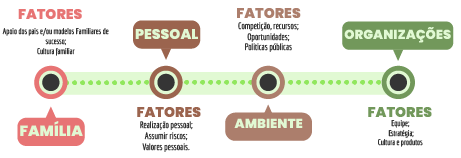
\includegraphics[scale=0.8]{Imagens/esquema_influencias_empreendedorismo.png}
\fonte{Adaptado de \cite{dornelas_empreendedorismo:_2005}}
\label{figura_2}
\end{figure}


Segundo \citeonline{bacich_metodologias_2018} a aprendizagem mais profunda e efetiva, requer espaços de prática frequentes (aprender fazendo) e de ambientes ricos em oportunidades se mostrando importante os estímulos interdisciplinares e multissensoriais, tais como o empreendedorismo acadêmico, utilizando para isto as metodologias ativas.Os mesmos autores definem as metodologias ativas como:

\begin{citacao}
Estratégias de ensino centradas na participação efetiva dos estudantes na construção do processo de aprendizagem, de forma flexível, interligada e híbrida. As metodologias ativas, num mundo conectado e digital, expressam-se por meio de modelos híbridos, com muitas possíveis combinações. A junção de metodologias ativas com modelos flexíveis e híbridos traz contribuições importantes para o desenho de soluções atuais para os aprendizes de hoje \cite{bacich_metodologias_2018}.
\end{citacao}

O ensino ativo do empreendedorismo acadêmico, apresenta-se também como uma potencial ferramenta para difusão e transferência de inovação e pesquisa realizadas por acadêmicos oriundos de laboratórios ou, departamentos onde a tecnologia se originou, \cite{guo_what_2019, abreu_nature_2013}, ou mesmo a busca de oportunidades e iniciativa utilizando os meios existentes no ambiente acadêmico. Os conteúdos necessários ao efetivo ensino do empreendedorismo vão além da oferta de apenas uma disciplina, é preciso que a instituição de ensino, a partir de novas práticas pedagógicas, transforme-se em também em uma instituição empreendedora \cite{campelli_empreendedorismo_2011}, que visualize a potencialidade da educação e promoção do comportamento empreendedor ao aluno com vistas a resolutividade de problemas \cite{degen_o_1989} e despertar da criatividade.

Diante da necessidade de solidificar o ensino empreendedor, que a \textit{Commission Enterprise and Industry Directorate-General} \cite{european_commission_best_2008} estruturou a educação empreendedora direcionada ao ensino superior em três objetivos, representados no modelo esquemático que pode ser visto na Figura \ref{figura_3}, em que se explica às três bases que estruturam os objetivos do ensino do Empreendedorismo no meio acadêmico. 

\begin{figure}[!htb]
\centering
\caption{\textbf{Pilares dos objetivos do ensino ao empreendedorismo.}}
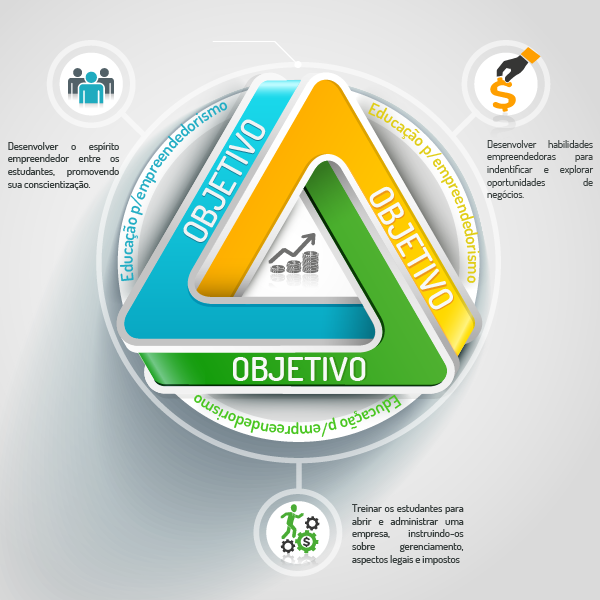
\includegraphics[scale=0.6]{Imagens/objetivos_educacao_empreendedora.png}
\fonte{Adaptado de \cite{european_commission_best_2008}}
\label{figura_3}
\end{figure}
\newpage

Como visto, ensino do empreendedorismo perpassa por diversas vertentes, porém, visando a associação de tais conteúdos aos técnicos científicos de forma interdisciplinar, e explorado neste trabalho a proposta de educação empreendedora que tem como base a Aprendizagem Baseada em Problemas (ABPR), a Aprendizagem Baseada em Projetos (ABP) \cite{bender_aprendizagem_2015} tendo como passos para elaboração dos conteúdos para o desenvolvimento de um empreendimento bem-sucedido os passos de \cite{aulet_empreendedorismo_2019} no livro: Empreendedorismo Disciplinado. 
Segundo \cite{bender_aprendizagem_2015} a ABP tem como objetivo o desenvolvimento do autoconhecimento com ênfase na perseverança, na imaginação, na criatividade, na inovação, para resolubilidade de problemas reais, sendo um importante o conteúdo que se aprende a fazer, mas, sobretudo, o que aprendido \cite{souza_disseminacao_2001}, de forma que a união de tais conhecimentos se some a um melhor desenvolvimento aos profissionais graduados que irão ao mercado de trabalho ou ao mundo dos negócios. Já que conhecimento científico promovido de forma interdisciplinar na graduação, além de repassar os conhecimentos técnicos, promove  uma considerável contribuição para se desenvolver o raciocínio independente, criativo e inovador buscamos nesta pesquisa uma abordagem que possa explorar todos os conteúdos de uma metodologia disciplinada e estruturada.


\section{Propriedade Intelectual no meio rural}

Toda criação advinda do intelecto humano, tais como música, produto, processo, nova cultivar, desenhos, artigos científicos, trabalhos literários ou artísticos constituem um ativo, bem ou direito \cite{costa_interseccao_2011}. Tais ativos sendo eles registrados ou não estão ligados diretamente ao seu autor/inventor sendo a propriedade  intelectual. Este direito vai muito além da inovação em si \cite{wipo_tratado_1970}, mas a relação entre o seu autor/inventor e sua respectiva criação intelectual. 


O conceito de Propriedade Intelectual é amplo e difere de país a país, em suma pode ser entendido como, à área do Direito que, garante a inventores ou responsáveis por qualquer produção do intelecto, seja nos domínios industrias, científicos, literários ou artísticos, o direito de obter, por um determinado período de tempo, recompensa pela própria criação \cite{aspi_aspi_2019}, é amparo legal e necessário para garantir que os investimentos em pesquisa e desenvolvimento retornem ao inventor, provocando um processo cíclico positivo, em que maiores investimentos em P&D seriam promovidos diante da concessão do monopólio temporário de exploração do invento \cite{lima_sauglobal_2017}. No Brasil a PI é composta por três grandes áreas: Propriedade Industrial, Direito do Autor e Suis generis, demais ramificações podem ser vistas na figura \ref{figura_4}.


\begin{figure}[h!]
\centering
\caption{\textbf{Modalidades da propriedade intelectual no Brasil}}
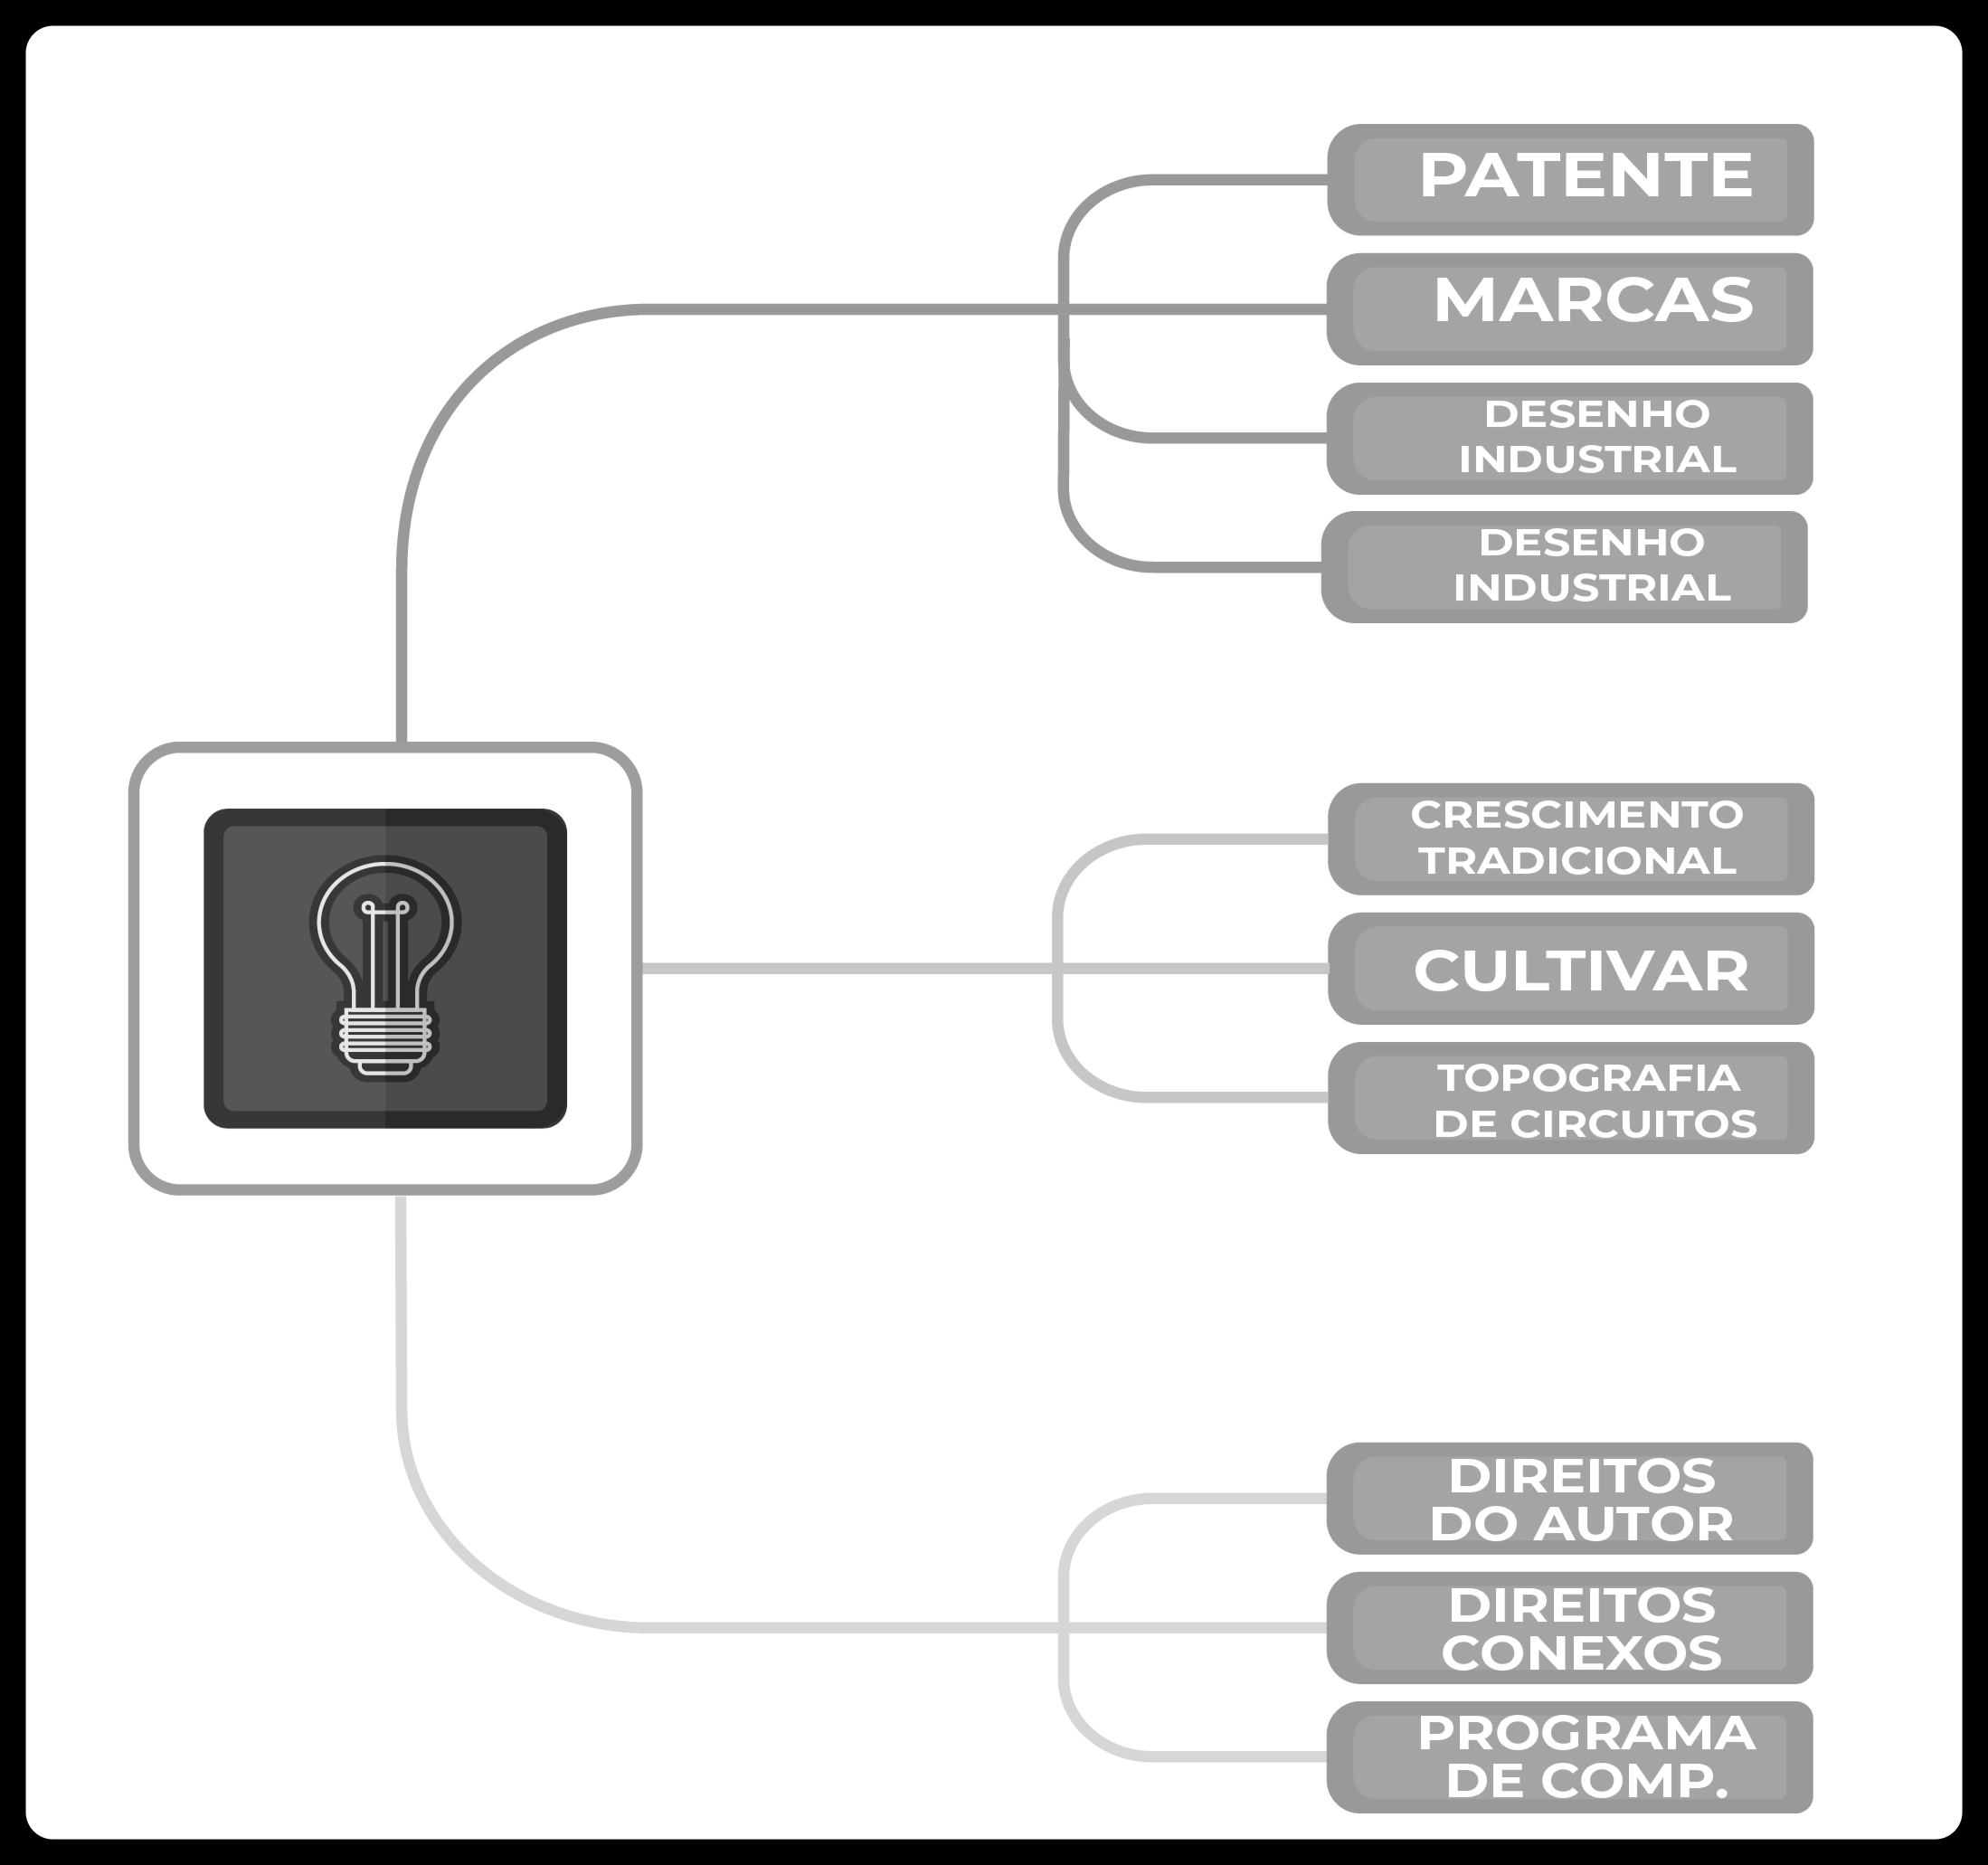
\includegraphics[scale=0.5]{Imagens/propriedade_intelectual.png}
\fonte{Adaptado de \cite{inpi_manual_2017}}
\label{figura_4}
\end{figure}
\newpage

Aliadas  às  ações  para  o  desenvolvimento  de  inovações, o inventor ou autor deve ter certa atenção as Propriedades Intelectuais que tangem seu produto, ou processo.  Sendo assim, é visível que há uma grande afinidade entre estes dois temas, principalmente os direitos que cabe ao meio industrial e do autor ligados a software. 

A crescente interação comercial,  financeira  e  tecnológica  entre  a  economia  e  seus  agentes  exigem  padrões  modernos  de  proteção  para  a  PI,  uma  vez  que  os  direitos sobre os nomes empresariais, tecnologias, \textit{designs}, marcas, entre outros, representam valiosos ativos das empresas e profissionais autores/inventores \cite{sherwood_propriedade_1992}. 


Diante de tais mudanças sobre o cenário do desenvolvimento tecnológico e das Propriedades Intelectuais (PI) inúmeras questões sobre o papel que os sistemas de registro e divulgação para PI desempenham no desenvolvimento e o incentivo à inovação \cite{segala_os_2016}. Os países que apresentam uma economia mais forte, dispõe de um sistema de proteção de propriedade mais robusto e confiável, concomitantemente, uma maior quantidade de registros e depósitos das mais variadas finalidades \cite{mueller_universidades_2014}.



